\begin{frame}{Architecture}{}
\centering
\begin{itemize}
    \item Gesture recognition
    \item Detecting user orientation
    \item Locating the user
\end{itemize}
\end{frame}


\begin{frame}{Gesture Recognition}{}
\centering
\begin{figure}
    \subfloat{
        \frame{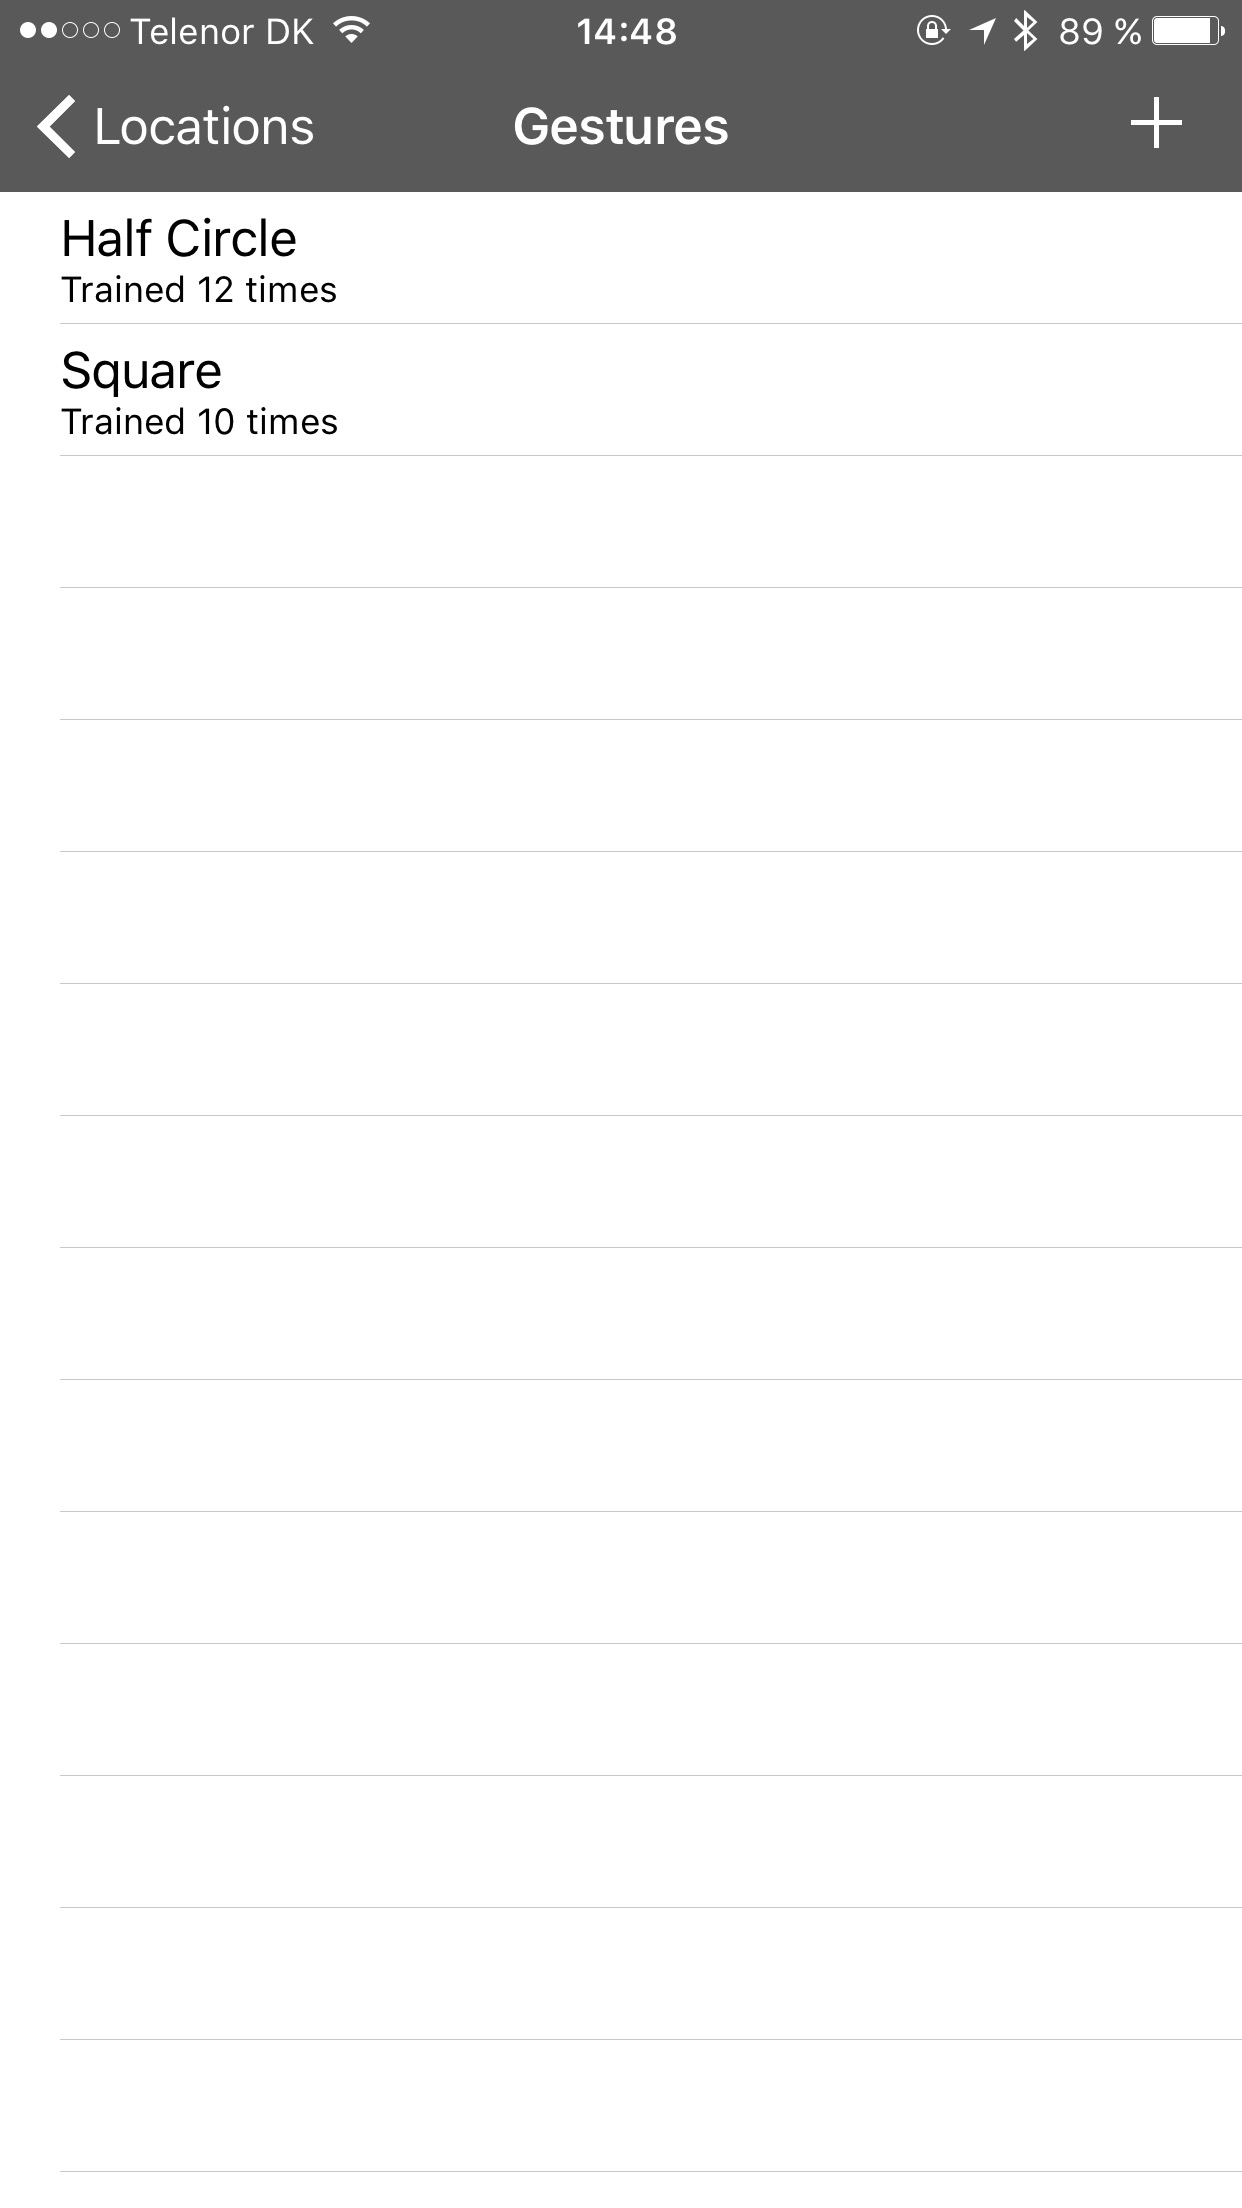
\includegraphics[width=0.3\textwidth]{../images/prototype-3-all-gestures}}
    }
    \subfloat{
        \frame{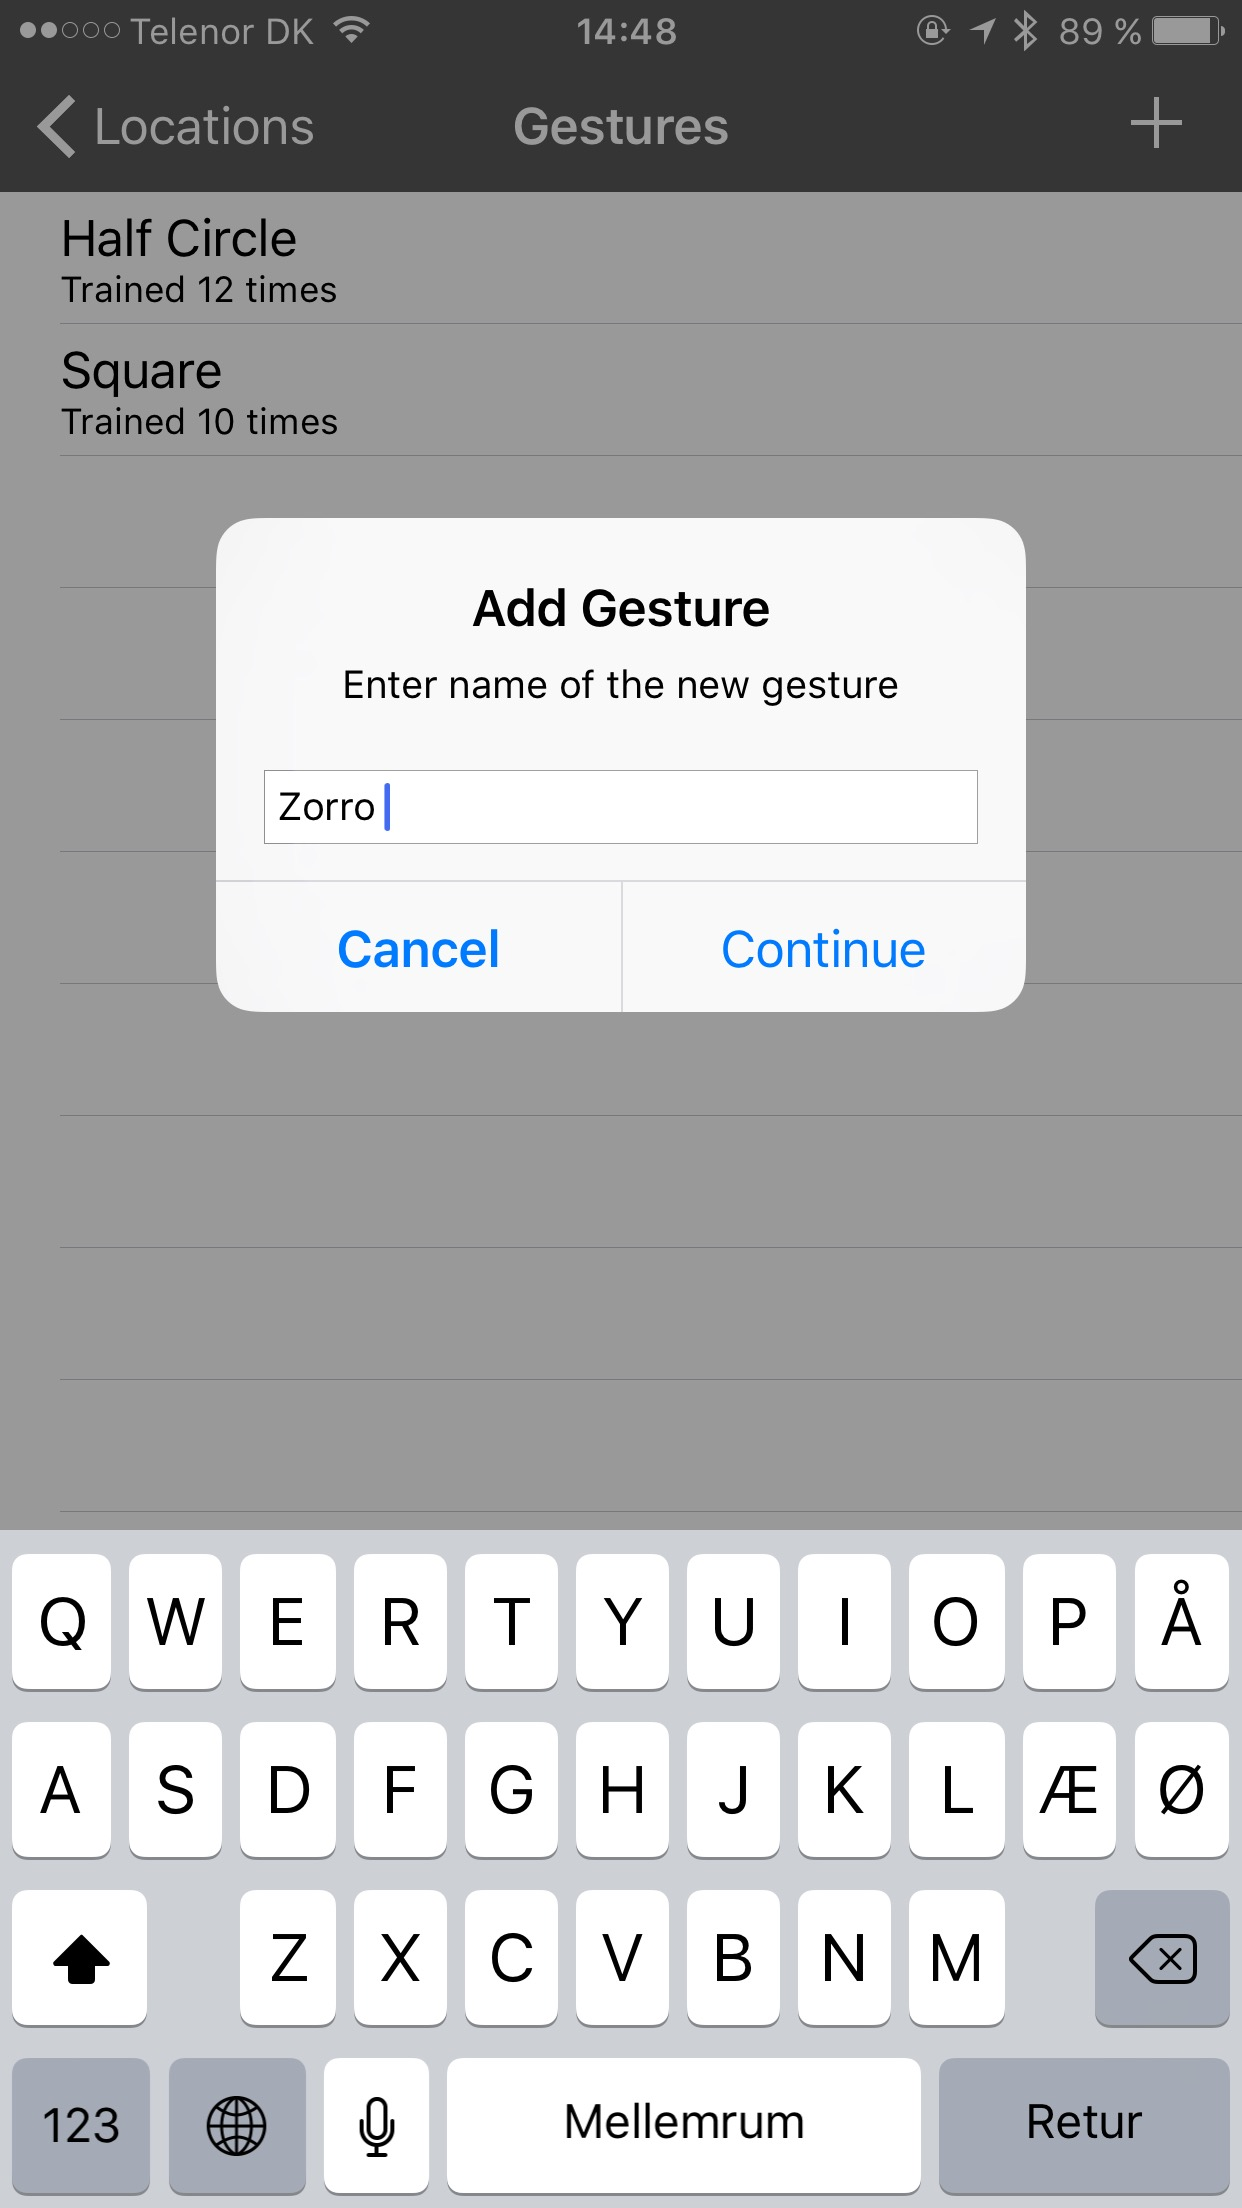
\includegraphics[width=0.3\textwidth]{../images/prototype-3-new-gesture}}
    }
    \subfloat{
        \frame{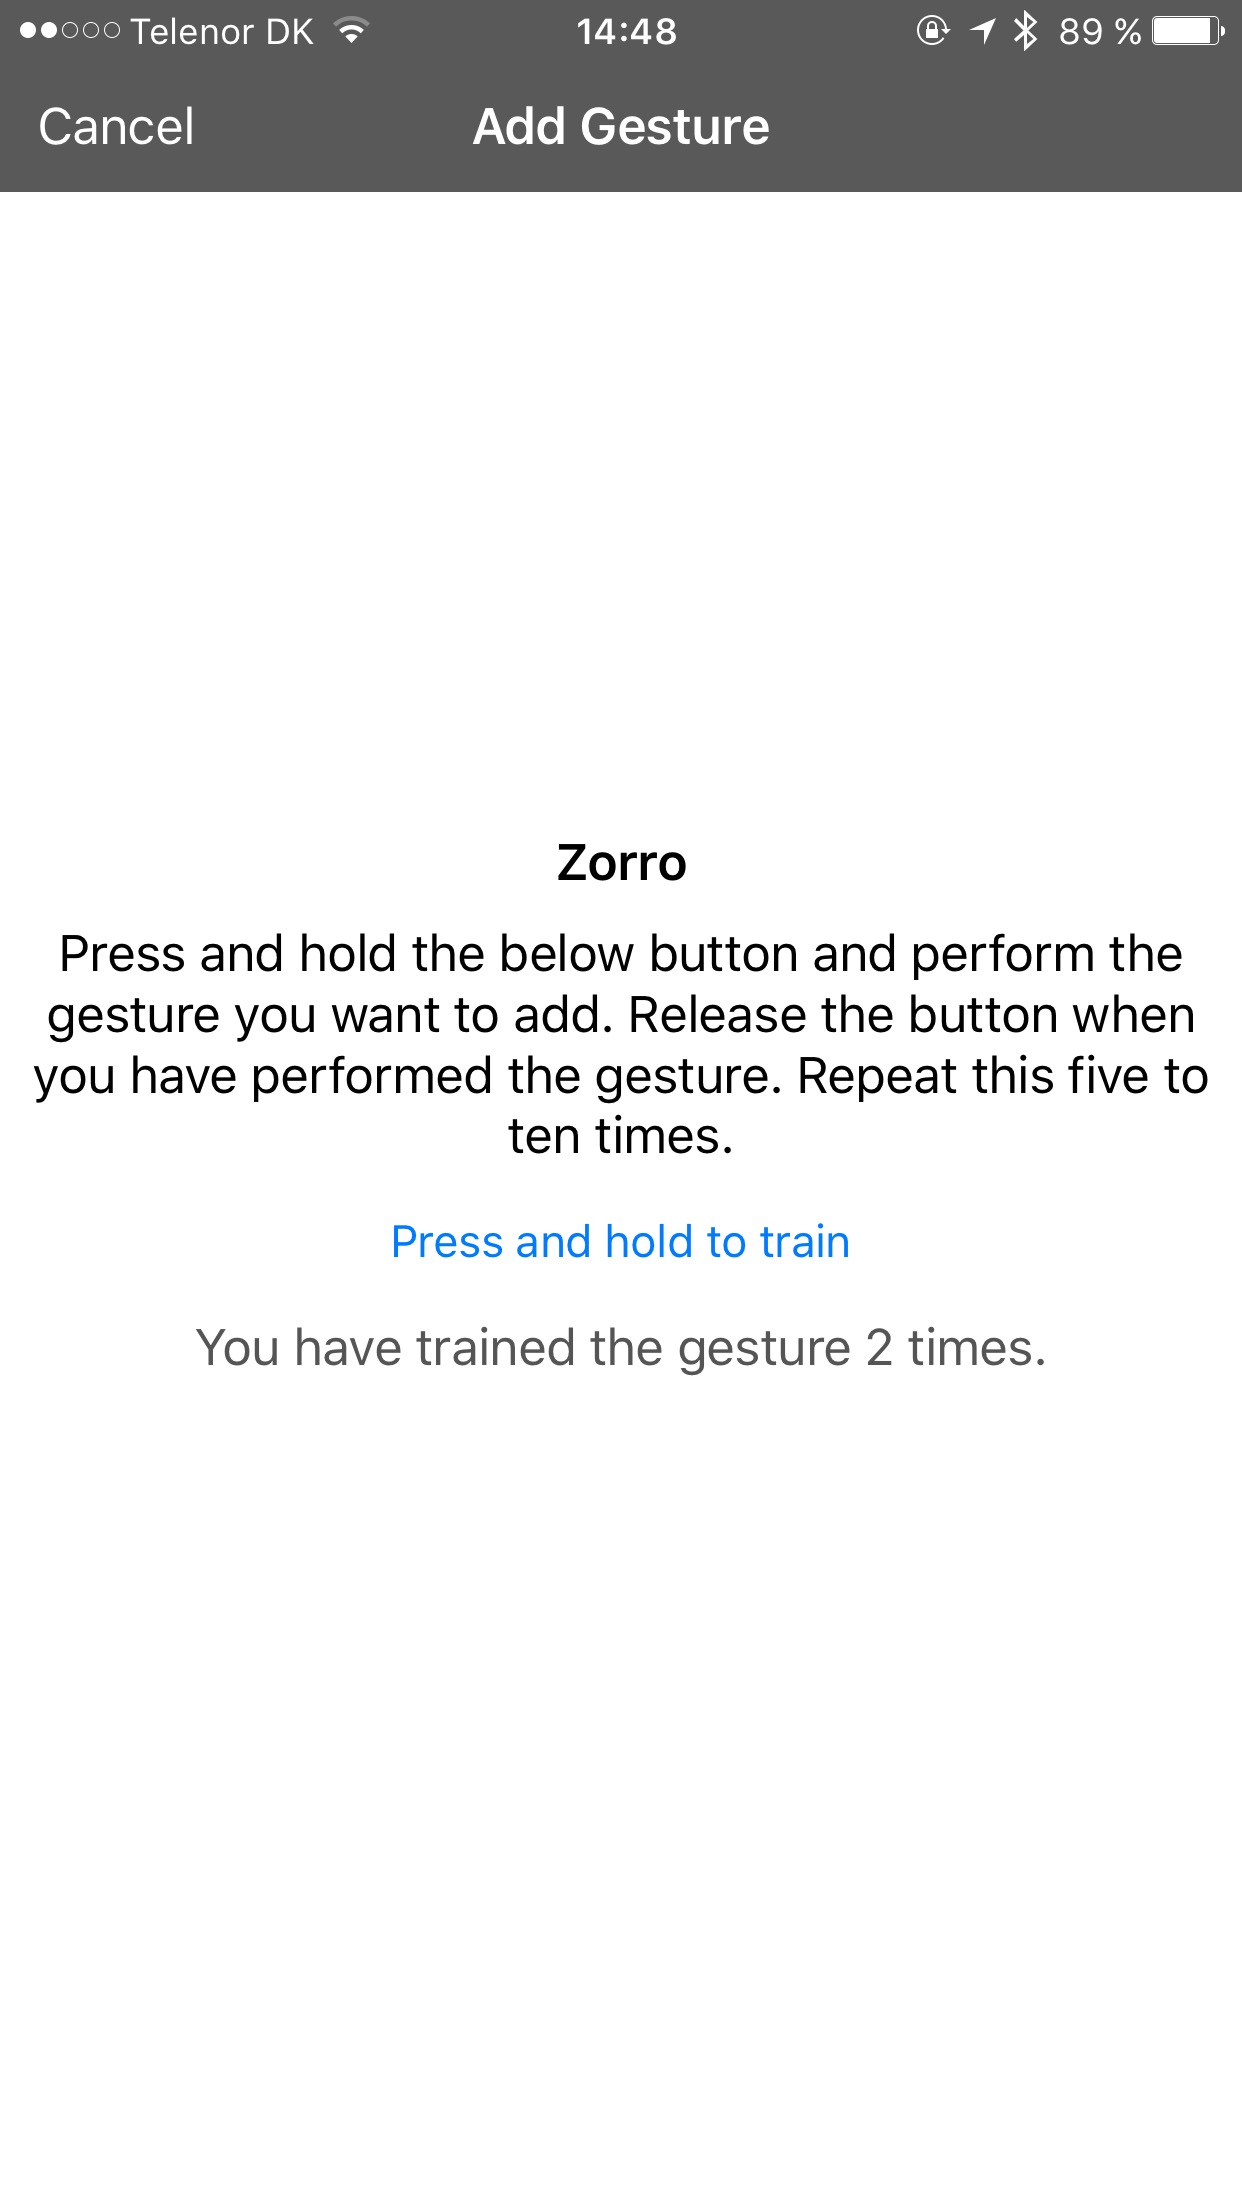
\includegraphics[width=0.3\textwidth]{../images/prototype-3-train-gesture}}
    }
    \caption{Screenshots showing the flow and interface for adding and training a new gesture in the third prototype.}
\label{fig:prototype3-gesture-screenshots}
\end{figure}
\end{frame}

\begin{frame}{Gesture Recognition}{Point Detection}
\centering
\begin{figure}
    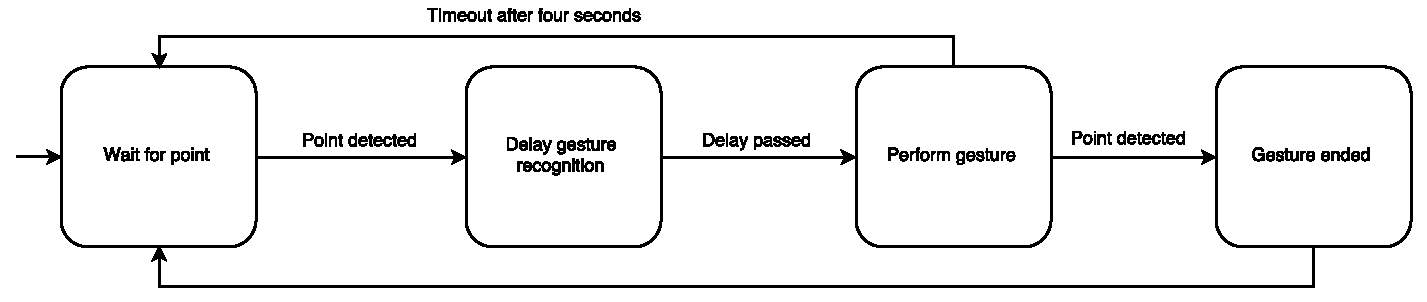
\includegraphics[width=\textwidth]{../images/point-to-gesture-state-diagram}
    \caption{State-chart diagram showing the relationship between a point and a gesture. A gesture always starts and ends with a point.}
\label{fig:point-to-gesture-state-diagram}
\end{figure}
\end{frame}